\documentclass[preprint,12pt, a4paper]{article}
\usepackage{amssymb}
\usepackage{hyperref}
\setlength{\parindent}{0pt}

\usepackage{pgfplots}
\usepackage{pgf-umlcd}

\usepackage[polish]{babel}
\usepackage[T1]{fontenc}
\usepackage{graphicx}
\graphicspath{ {./fig/} }

\usepackage{listings}
\usepackage{matlab-prettifier}
\usepackage{color}

%https://gist.github.com/sebald/3130827
\definecolor{dkgreen}{rgb}{0,0.6,0}
\definecolor{gray}{rgb}{0.5,0.5,0.5}
\definecolor{mauve}{rgb}{0.58,0,0.82}
\definecolor{gray}{rgb}{0.4,0.4,0.4}
\definecolor{darkblue}{rgb}{0.0,0.0,0.6}
\definecolor{lightblue}{rgb}{0.0,0.0,0.9}
\definecolor{cyan}{rgb}{0.0,0.6,0.6}
\definecolor{darkred}{rgb}{0.6,0.0,0.0}


\lstset{
  basicstyle=\ttfamily\footnotesize,
  columns=fullflexible,
  showstringspaces=false,
  numbers=left,                   % where to put the line-numbers
  numberstyle=\tiny\color{gray},  % the style that is used for the line-numbers
  stepnumber=1,
  numbersep=5pt,                  % how far the line-numbers are from the code
  backgroundcolor=\color{white},      % choose the background color. You must add \usepackage{color}
  showspaces=false,               % show spaces adding particular underscores
  showstringspaces=false,         % underline spaces within strings
  showtabs=false,                 % show tabs within strings adding particular underscores
  frame=none,                   % adds a frame around the code
  rulecolor=\color{black},        % if not set, the frame-color may be changed on line-breaks within not-black text (e.g. commens (green here))
  tabsize=2,                      % sets default tabsize to 2 spaces
  captionpos=b,                   % sets the caption-position to bottom
  breaklines=true,                % sets automatic line breaking
  breakatwhitespace=false,        % sets if automatic breaks should only happen at whitespace
  %title=\lstname,                   % show the filename of files included with \lstinputlisting;
                                  % also try caption instead of title  
  commentstyle=\color{gray}\upshape
}


\lstdefinelanguage{XML}
{
  morestring=[s][\color{mauve}]{"}{"},
  morestring=[s][\color{black}]{>}{<},
  morecomment=[s]{<?}{?>},
  morecomment=[s][\color{dkgreen}]{!--}{--},
  stringstyle=\color{black},
  identifierstyle=\color{lightblue},
  keywordstyle=\color{red},
  morekeywords={xmlns,xsi,noNamespaceSchemaLocation,type,id,x,y,source,target,version,tool,transRef,roleRef,objective,eventually}% list your attributes here
}

\lstdefinestyle{lstStyleLaTeX}{%
   ,language = [LaTeX]TeX%
   ,moretexcs={addplot,legend},
   ,keywordstyle=\color{cyan}
}

%https://gist.github.com/sebald/3130827
\usepackage{titlesec}
\titleformat*{\subparagraph}{\itshape\mdseries}

\usetikzlibrary{arrows.meta}
\tikzstyle{oneArrowStyle} = [-Stealth,line width = 1]
\tikzstyle{oneArrowinverseStyle} = [Stealth-,line width = 1]

\newcommand{\SoftwareName}{GTest }

\begin{document}

\renewcommand{\labelenumii}{\arabic{enumi}.\arabic{enumii}}

\tableofcontents


\section{Introduction}

The \SoftwareName (Multi-Criteria Decision Analysis MEthods Assessment through SimUlation REsearch) software includes a game module using the Unity game engine and a library created in the Matlab/Octave environment. The game module can be controlled using commands in which data is saved in XML format (fig.~\ref{Fig:architecture}). Responsible for visualizing the game board and controlling its course. By default, the game is configured to listen on port 55001. The default address (127.0.0.1) allows you to connect to the game only from the computer on which it is installed (however, this can be changed).

The library is intended to facilitate the creation of software in Matlab/Octave intended for testing decision support methods. Contains methods for preparing and formatting commands to be sent to the game. It also allows you to decode the answers received from the game. An additional option of the library is the conversion of tables to the tabular Latex environment format and a format that allows them to be read by the tikz package's charting module.

\begin{figure}
\begin{tikzpicture}
\node[rectangle,draw,minimum width = 3.5cm,minimum height = 1.5cm,label=above:{Player}] (r) at (-2.5,4.5) {Matlab/Octave};
\node[anchor=center,inner sep=0,label=above:{Game}] (game) at (4,4.5) {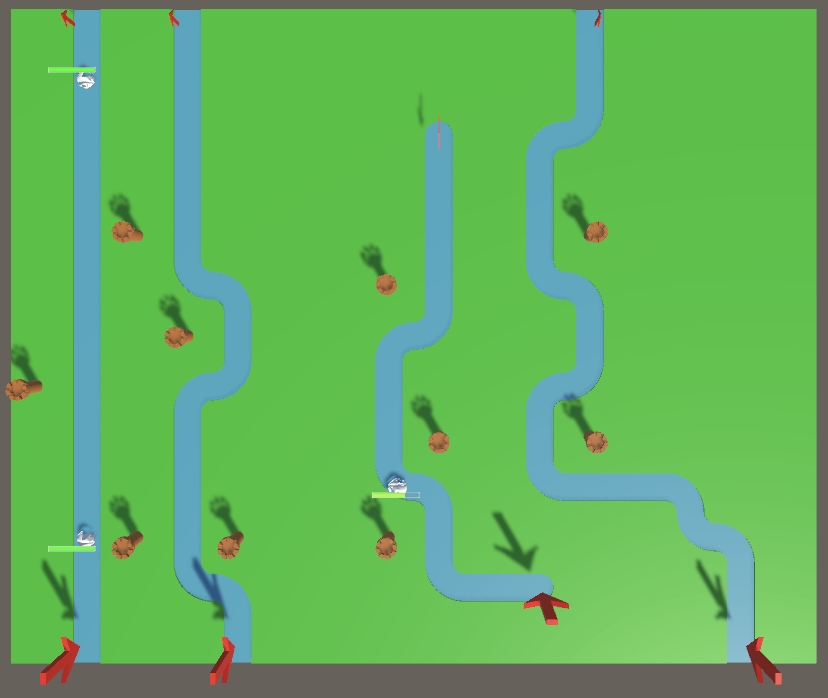
\includegraphics[width=3cm]{images/game.png}} ;
\node[anchor=center,inner sep=0, label=below:{Reports}] (tabaular) at (-2.5,1) {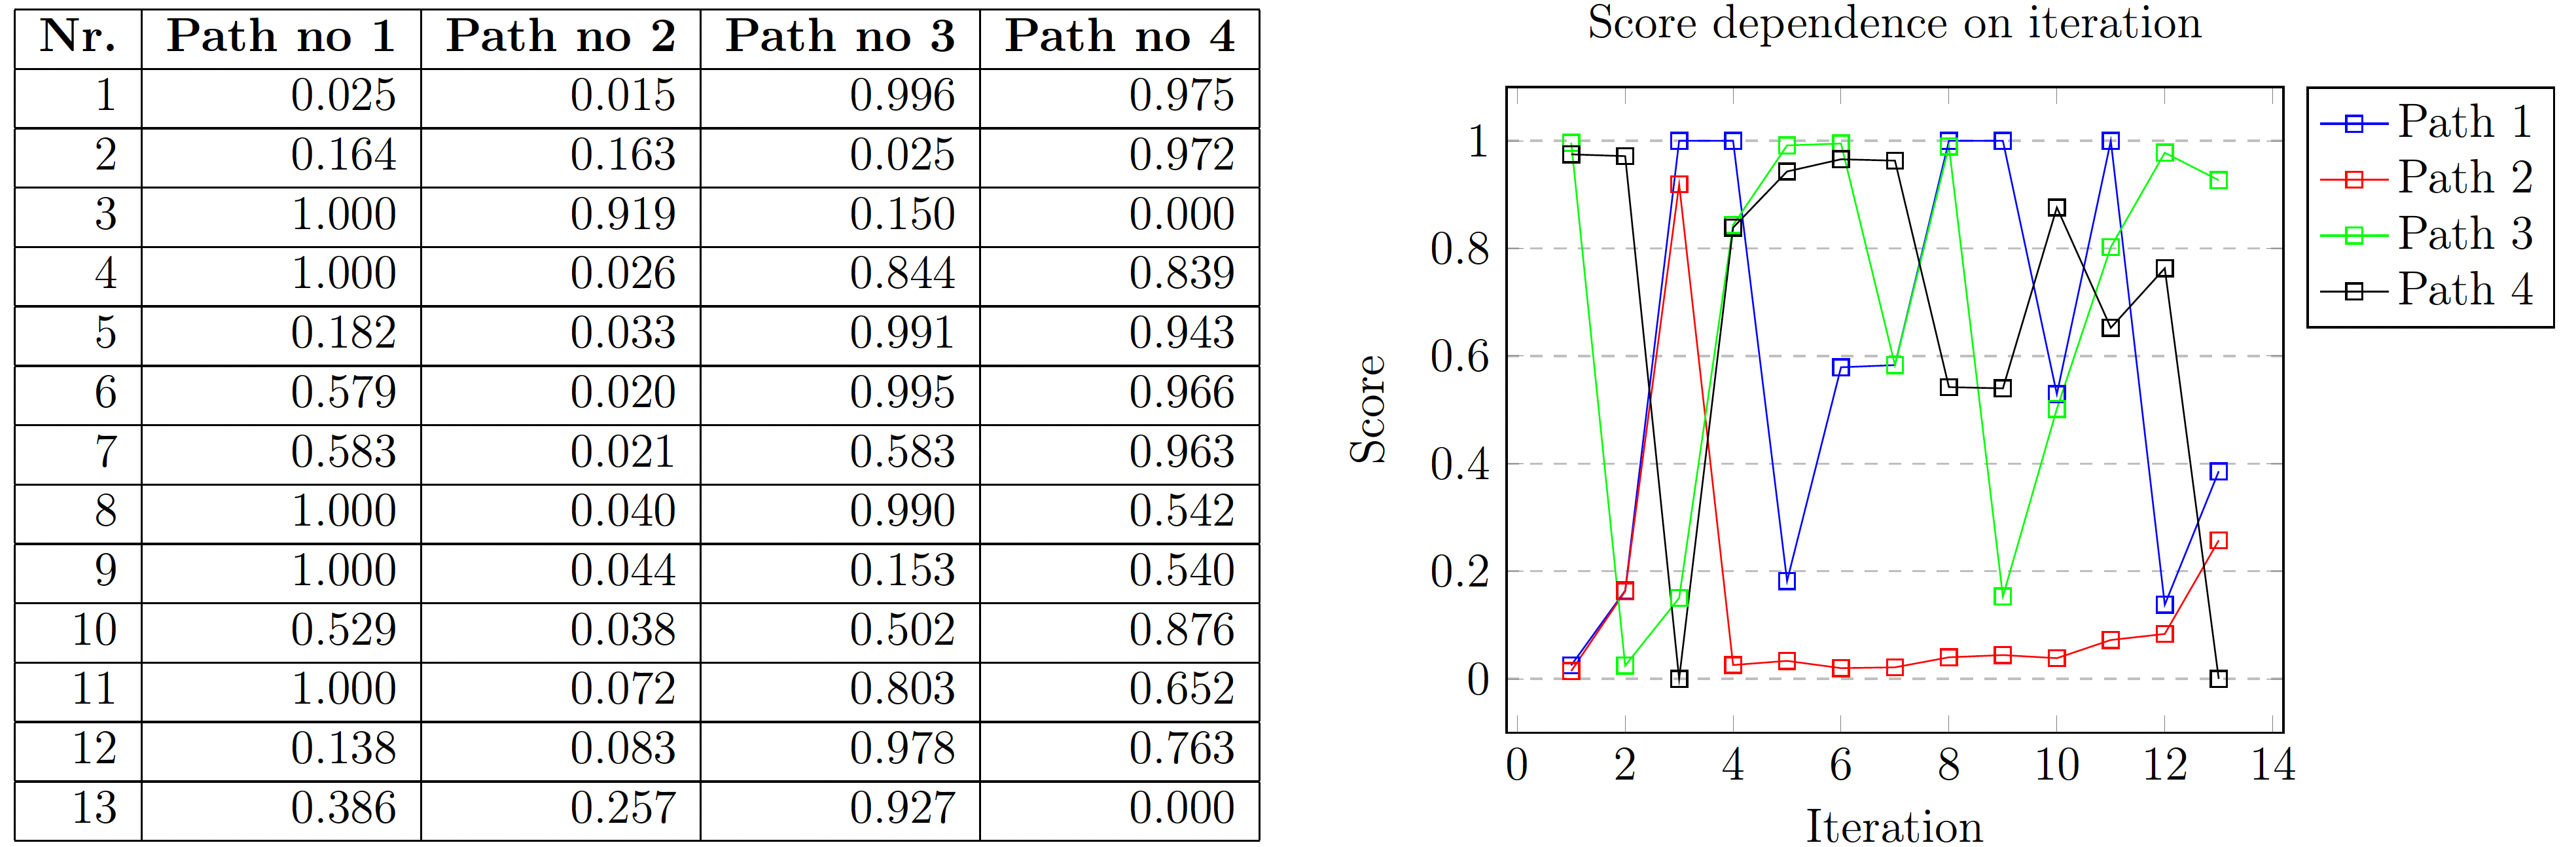
\includegraphics[height=2.5cm]{images/latexReports.png}};
\draw[oneArrowinverseStyle] (r.east) + (0,-0.1) -- ++(3.3,-0.1) node[midway,below]{Answer};
\draw[oneArrowStyle] (r.east) + (0,0.1) -- ++(3.3,0.1) node[midway,above]{Command};
\draw[oneArrowStyle] (r) -- (tabaular);

\end{tikzpicture}

\caption{System architecture}
\label{Fig:architecture}
\end{figure}

\section{Game}

Gra jest wykonana w środowisku Unity. Należy ona do typu tower defense. Plansza gry składa się z tiles będących trójwymiarowymi modelami dzielącymi się na dwie kategorie: ziemia i droga. Jest jeden tile typu ziemia i pięć tiles typu droga (fig.~\ref{Fig:tiles}).

\begin{figure}
\begin{tikzpicture}
\node[anchor=center,inner sep=0, label=below:{Ground}] at (-4,3) {
\includegraphics[width=2cm]{images/tileGround.png}};
\node[anchor=center,inner sep=0, label=below:{Water}] at (-4,1) {
\includegraphics[width=2cm]{images/tileWater.png}};
\node[anchor=center,inner sep=0,label=below:{Straight}] (tikz) at (-1.5,1) {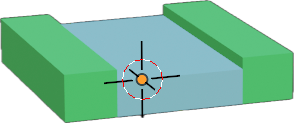
\includegraphics[width=2cm]{images/tileWaterStraight.png}};
\node[anchor=center,inner sep=0,label=below:{Curve}] (tikz) at (1,1) {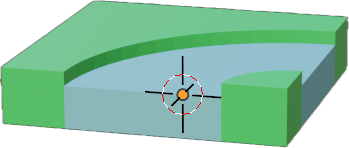
\includegraphics[width=2cm]{images/tileWaterCurve.png}};
\node[anchor=center,inner sep=0,label=below:{Intersection 1}] (tikz) at (3.5,1) {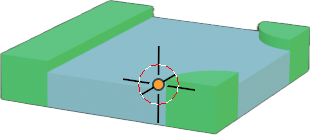
\includegraphics[width=2cm]{images/tileWaterIntersection1.png}};
\node[anchor=center,inner sep=0,label=below:{Intersection 2}] (tikz) at (6,1) {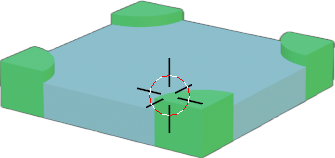
\includegraphics[width=2cm]{images/tileWaterIntersection2.png}};
\end{tikzpicture}

\caption{Modele tiles}
\label{Fig:tiles}
\end{figure}  

Na rysunku~\ref{Fig:changeTiles} pokazano w którym miejscu w interfejsie edytora Unity należy zmienić modele tiles (o ile to będzie istniała taka  potrzeba). Górne zaznaczenie pokazuje miejsce zmiany modelu tile typu ziemia. Dolne zaznaczenie pokazuje miejsce zmiany pierwszego modelu tile typu droga. Pozostałe znajdują się w WaterStraight, WaterCurve itd. Elementy WaterBegin, WaterBeginEnd itp. są kombinacją modeli z rysunku~\ref{Fig:tiles} ze strzałkami. 

\begin{figure}
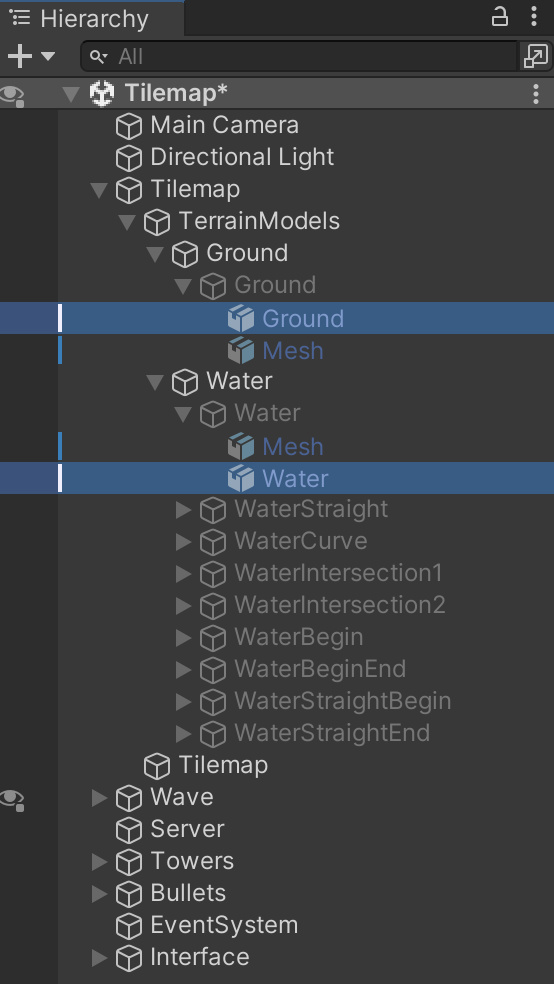
\includegraphics[width=5cm]{images/changeTiles.png}
\caption{Zmiana modeli tiles}
\label{Fig:changeTiles}
\end{figure}  

Na podobnej zasadzie można zmieniać model przeciwników i wież. Miejsce zmian modeli są pokazane na rysunkach~\ref{Fig:changeEnemy} i ~\ref{Fig:changeTower}.

\begin{figure}
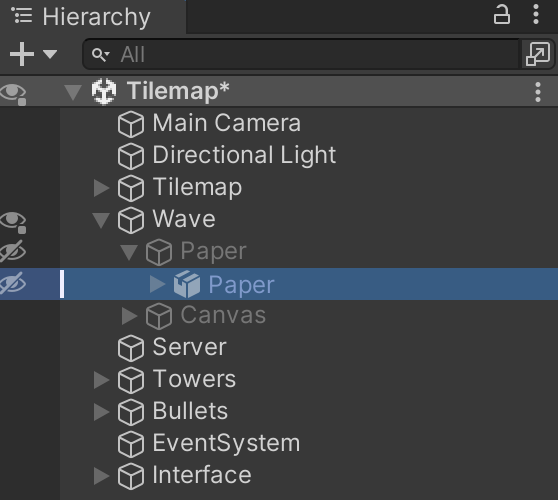
\includegraphics[width=5cm]{images/changeEnemy.png}
\caption{Zmiana modelu przeciwnika}
\label{Fig:changeEnemy}
\end{figure}  


\begin{figure}
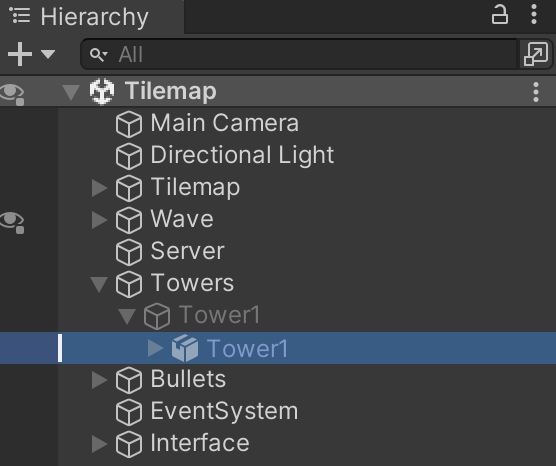
\includegraphics[width=5cm]{images/changeTower.png}
\caption{Zmiana modelu wieży}
\label{Fig:changeTower}
\end{figure}  

Rysunek~\ref{Fig:enemyParameters}  przedstawia miejsce w którym w edytorze Unity można zmienić parametry przeciwników:
\begin{itemize}
\item Speed -- prędkość poruszania się,
\item Start health -- start health,
\item Armour -- wartość odejmowana od zadanych obrażeń (powoduje niewrażliwość na pociski, które mają niższą liczbę zadawanych obrażeń od Armour),
\item Coins -- liczba coins potrzebna do utworzenia przeciwnika,
\item Destroy Coins -- liczba coins jaką otrzymują wieże za zabicie przeciwnika,
\item Coins To End -- liczba coins jaką otrzymują przeciwnicy jeżeli przeciwnik dotrze do punktu końcowego,
\item Count -- liczba dostępnych przeciwników (-1 oznacza niegraniczoną liczbę przeciwników).  
\end{itemize}

\begin{figure}
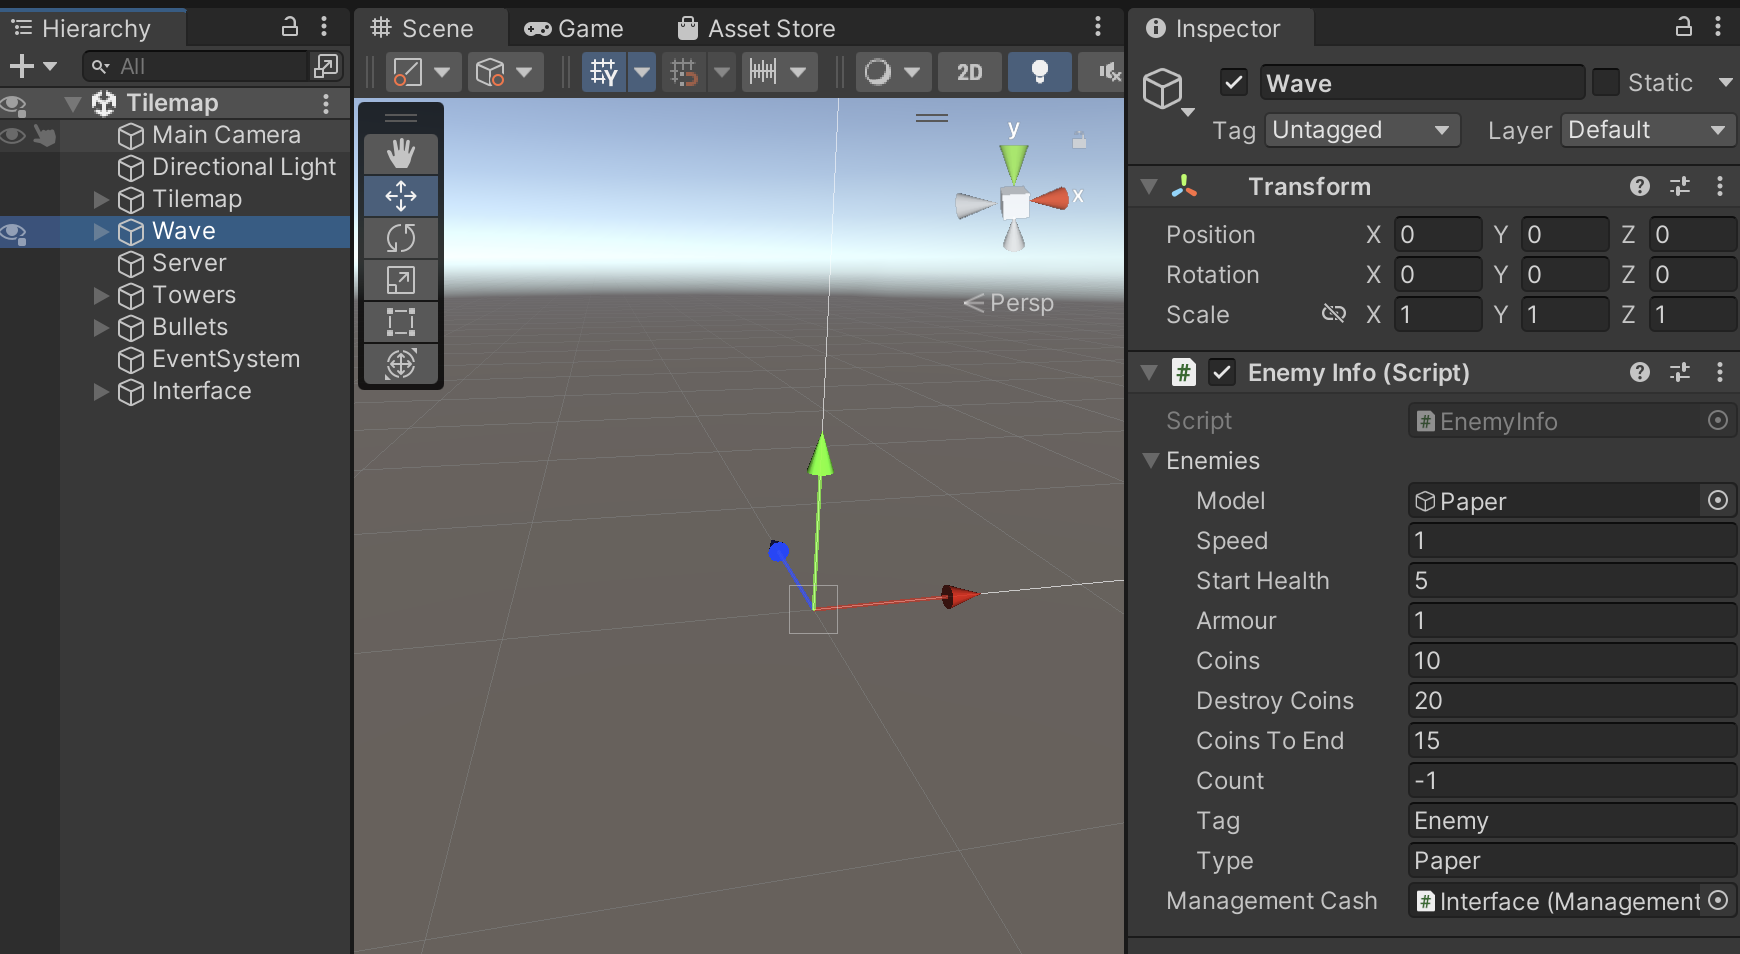
\includegraphics[width=15cm]{images/enemyParameters.png}
\caption{Zmiana parametrów przeciwników}
\label{Fig:enemyParameters}
\end{figure}  

Rysunek~\ref{Fig:towerParameters}  przedstawia miejsce w którym w edytorze Unity można zmienić parametry wież:
\begin{itemize}
\item Speed -- prędkość obrotu,
\item Rate Od Fire -- szybkostrzelność,
\item Bullet Strength -- liczba zadawanych obrażeń,
\item Force -- siła wystrzelenia pocisku przekładająca się na jego zasięg,
\item Coins -- liczba coins potrzebna do utworzenia wieży,
\item Count -- liczba dostępnych wież (-1 oznacza niegraniczoną liczbę wież).  
\end{itemize}

\begin{figure}
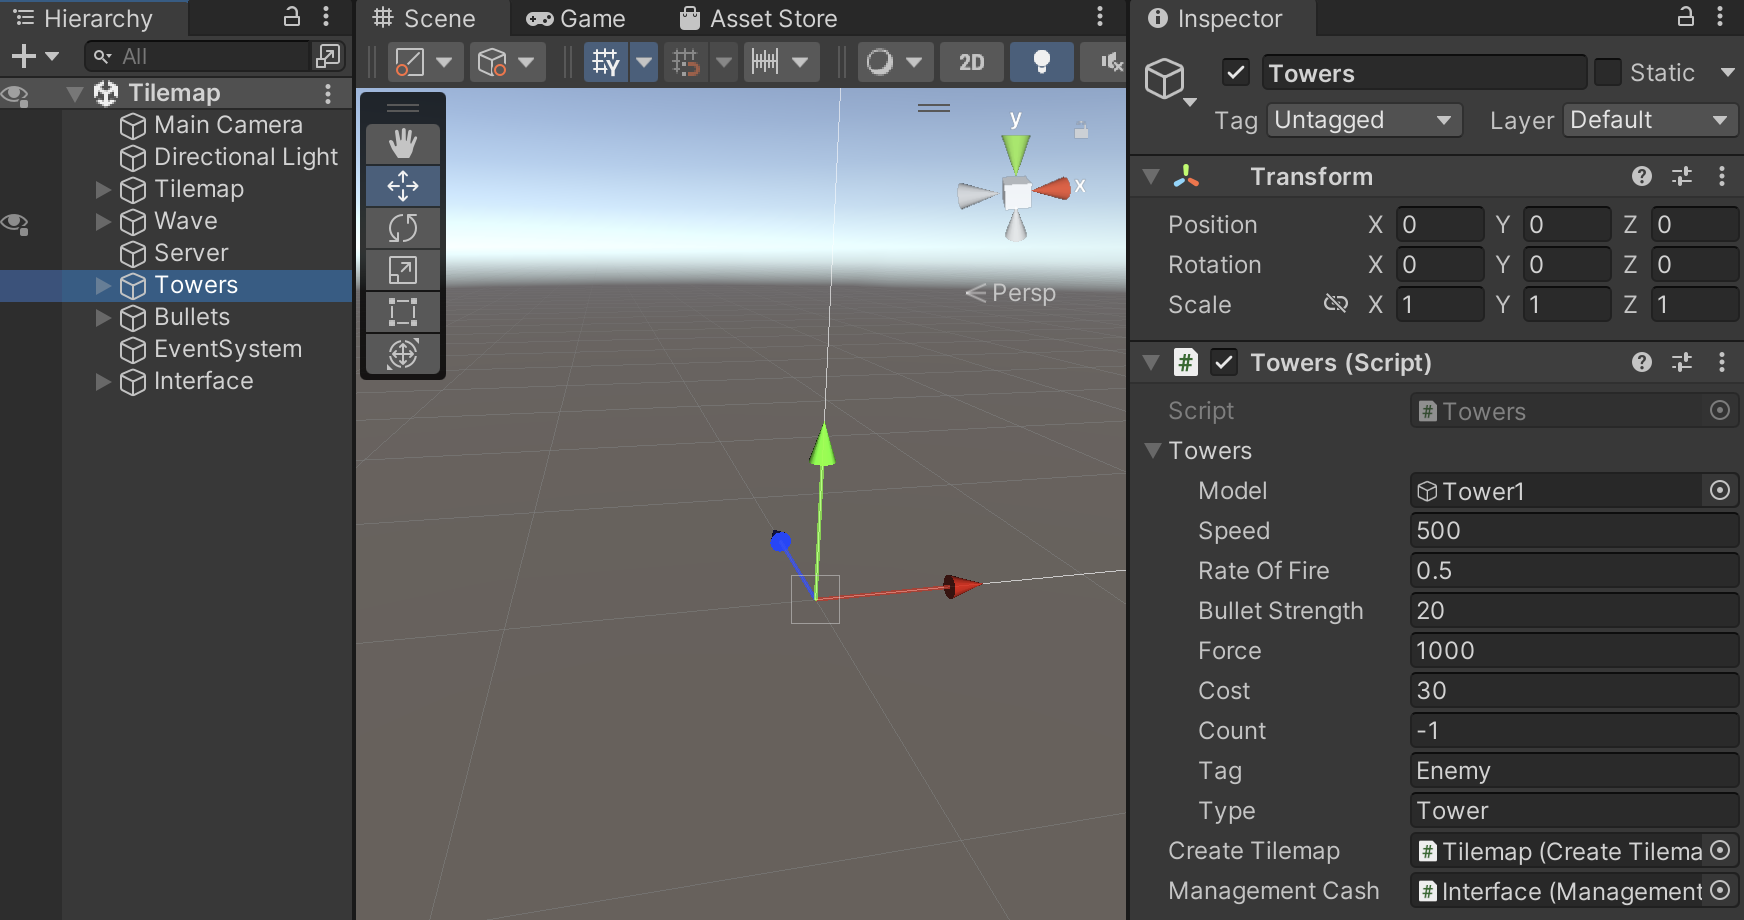
\includegraphics[width=15cm]{images/towerParameters.png}
\caption{Zmiana parametrów wież}
\label{Fig:towerParameters}
\end{figure}  

Rysunek~\ref{Fig:startCoins}  przedstawia miejsce w którym w edytorze Unity można zmienić początkową liczbę coins:
\begin{itemize}
\item Start Coins --  początkowa liczba coins wież; 
\item Start Enemy Coins --  początkowa liczba coins przeciwników. 
\end{itemize}


\begin{figure}
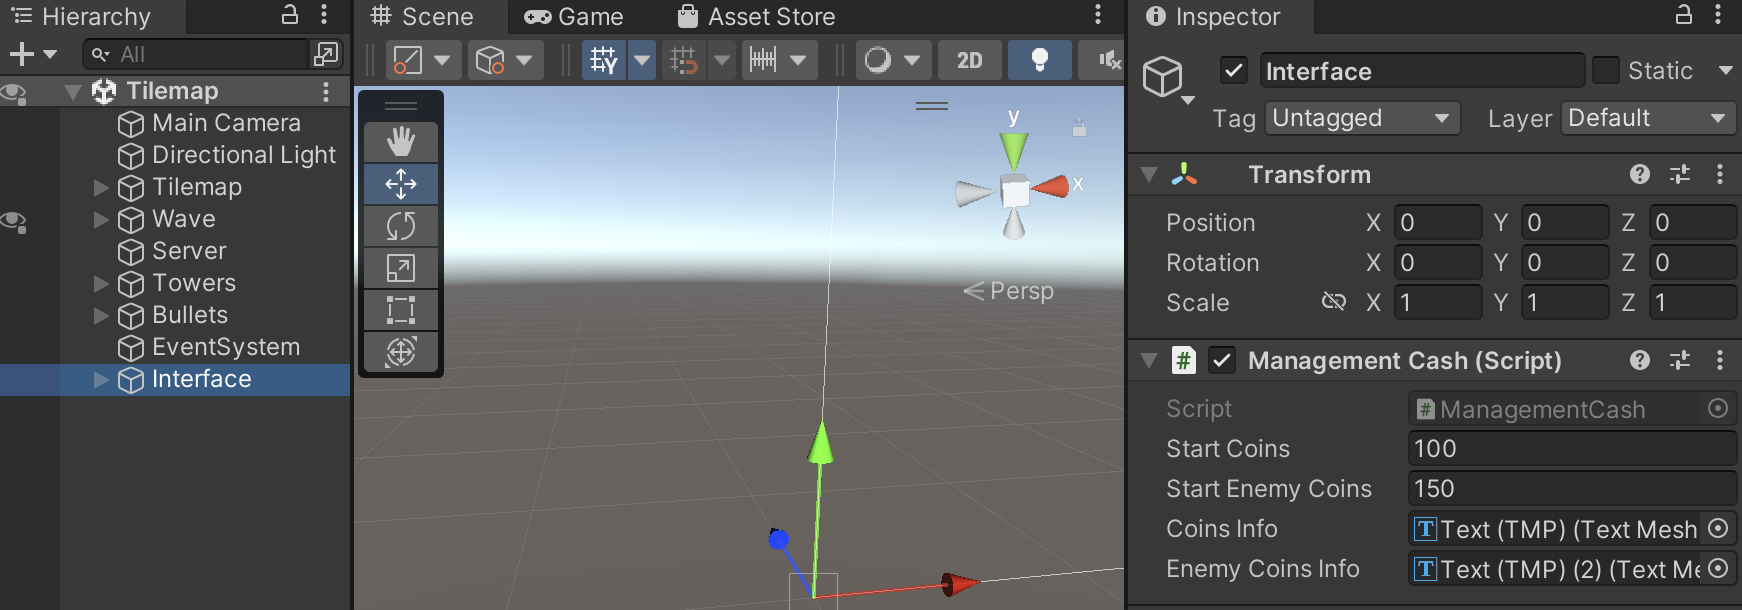
\includegraphics[width=15cm]{images/startCoins}
\caption{Początkowe coins}
\label{Fig:startCoins}
\end{figure} 

Rysunek~\ref{Fig:serverParameters}  przedstawia miejsce w którym w edytorze Unity można zmienić parametry serwera: 
\begin{itemize}
\item IP Adress --  adres ip serwera (127.0.0.1 oznacza, że serwer będzie dostępny tylko dla oprogramowania zainstalowanego na tym samym komputerze co gra); 
\item Port --  port na którym nasłuchuje serwer. 
\end{itemize}

\begin{figure}
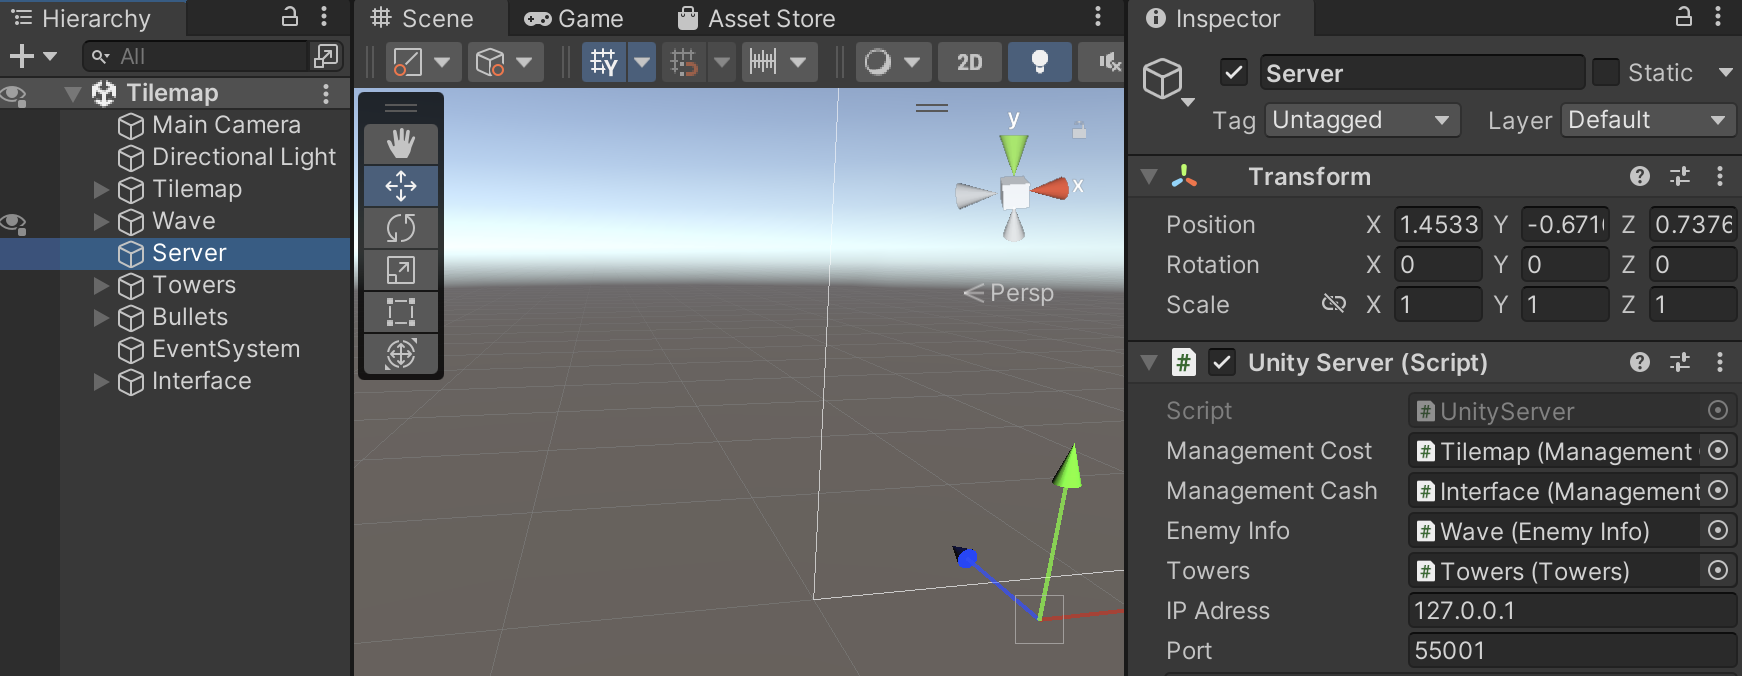
\includegraphics[width=15cm]{images/serverParameters.png}
\caption{Parametry serwera komunikacyjnego}
\label{Fig:serverParameters}
\end{figure} 

Planszę gry stanowi zbiór $n \times m$ tiles mających podstawę kwadratu. $n$ i $m$ to odpowiednio szerokość i wysokość planszy wyrażona w długościach boku kwadratu będącego podstawą tile. Przykładowy XML  definiujący planszę gry:
\lstinputlisting[language=XML]{xml/tilemap.xml}

Po wysłaniu danych, zwracana jest informacja w postaci XML. W przypadku definicji planszy gry zwracane są dane XML z informacją o poprawności (lub nie) informacji przekazanej do serwera:
\lstinputlisting[language=XML]{xml/tilemapResponse.xml}

XML definiujący parametry przeciwników:
\lstinputlisting[language=XML]{xml/enemy.xml}

Po zdefiniowaniu parametrów zwracana jest informacja o poprawności wykonania komendy (analogiczna jak w przypadku tilemap). 

XML definiujący parametry wież:
\lstinputlisting[language=XML]{xml/tower.xml}

Po definiowaniu parametrów zwracana jest informacja o poprawności wykonania komendy (analogiczna jak w przypadku tilemap). 

Utworzenie przeciwnika i wypuszczenie go wybraną ścieżką:
\lstinputlisting[language=XML]{xml/addEnemy.xml}

Po utworzeniu przeciwnika zwracana jest informacja o poprawności wykonania komendy (analogiczna jak w przypadku tilemap). 

XML powodujący dodanie nowej wieży:
\lstinputlisting[language=XML]{xml/addTower.xml}

Po dodaniu nowej wieży zwracana jest informacja o poprawności wykonania komendy (analogiczna jak w przypadku tilemap). 

Żądanie przesłania informacji o ścieżkach:
\lstinputlisting[language=XML]{xml/GetChoiceOfPathData.xml}

Zwracana przez serwer informacja:
\lstinputlisting[language=XML]{xml/GetChoiceOfPathDataResponse.xml}

Żądanie przesłania szczegółowych informacji o stanie gry:
\lstinputlisting[language=XML]{xml/LevelData.xml}

Zwracana przez serwer informacja:
\lstinputlisting[language=XML]{xml/LevelDataResponse.xml}

\section{Biblioteka}

Biblioteka jest stanowi zbiór funkcji wspomagających komunikację z grą oraz tworzenie tabel i wykresów. Funkcje te działają zarówno w środowisku Matlab jak i Octave.

\paragraph{SendData} \hspace{0pt} \\
Sending data to the server.

%\subparagraph{Syntax}\hspace{0pt} \\
\begin{lstlisting}[style=Matlab-editor]
txt = SendData(IPAddressSend,portSend,data,name, args)
\end{lstlisting}

Description:
\begin{itemize}
\item  IPAddressSend -- server ip address,
\item  portSend -- server port,
\item  data -- data packet sent to the server,
\item  name  -- control information sent to the server,
\item  args  -- arguments related to control information.
\end{itemize}

Returns the response from the server in xml format.

\paragraph{NumberToName} \hspace{0pt} \\
Zamienia tablicę dwuwymiarową w tablicę struktur. Replacing numbers representing field types with their names.
\begin{lstlisting}[style=Matlab-editor]
result = NumberToName(array, names)
\end{lstlisting}

Description:
\begin{itemize}
\item  array -- a table containing information about the map,
\item  names -- map field names.
\end{itemize}

Returns a table containing information about the map.

\paragraph{ChangeBeginEnd} \hspace{0pt} \\
Marking the beginnings and ends of paths.
\begin{lstlisting}[style=Matlab-editor]
result = ChangeBeginEnd(array)
\end{lstlisting}

Description:
\begin{itemize}
\item  array -- a table containing information about the map.
\end{itemize}

Returns a table containing information about the map.

\paragraph{TilemapToXML} \hspace{0pt} \\
Map conversion from an array to xml format.
\begin{lstlisting}[style=Matlab-editor]
txt = TilemapToXML(tilemap)
\end{lstlisting}

Description:
\begin{itemize}
\item  tilemap -- map in the form of an array.
\end{itemize}

Returns a map saved in xml format.

Przykład przesłania do gry polecenia utworzenia planszy:
\begin{lstlisting}[style=Matlab-editor]
%Adres serwera
IPAddressSend = '127.0.0.1';
%Port na ktorym nasluchuje serwer
portSend = 55001;
%Tablica reprezentujaca plansze gry w ktorej liczby reprezentuja typy tiles (1 - ziemia, 2 - woda bedaca elementem sciezki ruchu przeciwnikow, 3 - poczatek sciezki, 4 - koniec sciezki) 
tilemap = [1	3	1	3	1	1	1	1	1	1	1	3	1	1	1 1;
           	1	2	1	2	1	1	1	1	1	1	1	2	1	1	1 1;
           	1	2	1	2	1	1	1	1	3	1	2	2	1	1	1 1;
           	1	2	1	2	1	1	1	1	2	1	2	1	1	1	1 1;
           	1	2	1	2	1	1	1	1	2	1	2	1	1	1	1 1;
           	1	2	1	2	2	1	1	1	2	1	2	2	1	1	1 1;
           	1	2	1	1	2	1	1	2	2	1	1	2	1	1	1 1;
           	1	2	1	2	2	1	1	2	1	1	2	2	1	1	1 1;
           	1	2	1	2	1	1	1	2	1	1	2	1	1	1	1 1;
           	1	2	1	2	1	1	1	2	2	1	2	2	2	2	1 1;
           	1	2	1	2	1	1	1	1	2	1	1	1	1	2	2 1;
           	1	2	1	2	2	1	1	1	2	2	4	1	1	1	2 1;
           	1	4	1	1	4	1	1	1	1	1	1	1	1	1	4 1];
%Nazwy typow tiles. Pozycja w tablicy odpowiada numerowi z tablicy tilemap
names{1} = 'Ground';
names{2} = 'Water';
names{3} = 'Begin';
names{4} = 'End';
%Obrot tablicy tak aby orientacja tablicy odpowiadala orientacji planszy w grze
tilemap = rot90(rot90(rot90(tilemap)));
% Zamiana tablicy na tablice struktur z nazwami tiles zamiast numerow
tilemapNames = NumberToName(tilemap,names);
%Zamiana nazw tiles Begin i End na Water. Przypisanie tym tiles oznaczenia poczatku lub konca sciezki.
tilemapNames = ChangeBeginEnd(tilemapNames);
%Zamiana tablicy sturktur na tekst w formacie xml.
txt = TilemapToXML(tilemapNames);
%Wyslanie polecenia utworzenia nowej planszy (Tilemap) oraz danych w formacie xml do gry.
SendData(IPAddressSend,portSend,txt,'Tilemap',[]);
\end{lstlisting}

\paragraph{ParseXML} \hspace{0pt} \\
Parses text containing xml.
\begin{lstlisting}[style=Matlab-editor]
result = ParseXML(data)
\end{lstlisting}

Description:
\begin{itemize}
\item data -- a text array containing data in xml format.
\end{itemize}

Returns an array of structures whose structure reflects the structure of the XML data, the field names are the names of the XML elements.

Przykład odczytania i zdekodowania pliku xml:
\begin{lstlisting}[style=Matlab-editor]
%Odczytanie pliku xml
dataTower = fileread('towers.xml');
%Konwersja pliku xml
dataTower = ParseXML(dataTower);
\end{lstlisting}

Zawartość pliku towers.xml:
\lstinputlisting[language=XML]{xml/towersBib.xml}

Plik towers.xml zawiera współrzędne wież i ich numery porządkowe. Przykład dostępu do tych danych:
\begin{lstlisting}[style=Matlab-editor]
x=dataTower.Answer.TowerCoordinates{1}.Element{i}.x;
y=dataTower.Answer.TowerCoordinates{1}.Element{i}.y;
no=dataTower.Answer.TowerCoordinates{1}.Element{i}.no;
\end{lstlisting}

\paragraph{GetVectorFromCell} \hspace{0pt} \\
Reading a data vector from a selected field of the structure array.
\begin{lstlisting}[style=Matlab-editor]
res = GetVectorFromCell(data, field)
\end{lstlisting}

Description:
\begin{itemize}
\item data -- structure array,
\item field -- read structure fields.
\end{itemize}

Returns a data vector.

Przykład odczytania współrzędnych x wież jako tablicy:
\begin{lstlisting}[style=Matlab-editor]
%Odczytanie pliku xml
dataTower = fileread('towers.xml');
%Konwersja pliku xml
dataTower = ParseXML(dataTower);
%Odczytanie wspolrzednych x wiez jako tablicy
x = GetVectorFromCell(dataTower.Answer.TowerCoordinates{1}.Element,'x');
\end{lstlisting}

Zawartość pliku towers.xml:
\lstinputlisting[language=XML]{xml/towersBib.xml}

\paragraph{SetEnemies} \hspace{0pt} \\
Creating information in the form of XML about a specific type of opponent.
\begin{lstlisting}[style=Matlab-editor]
txt = SetEnemies(count,speed,startHealth,armour,cost,destroyCoins,coinsToEnd,type,tag)
\end{lstlisting}

Description:
\begin{itemize}
\item count -- maximum number of opponents,
\item speed -- opponent's speed,
\item startHealth -- opponent's starting life value,
\item armour -- enemy's armor (bullet resistance),
\item cost -- the cost of creating and sending an enemy,
\item destroyCoins -- profit for the tower manager for shooting down an enemy,
\item coinsToEnd -- gain for the opponent's manager if he reaches the end of the path,
\item type -- opponent type,
\item tag -- name of the object type.
\end{itemize}

Returns information saved in xml format.

Przykład przesłania do gry polecenia utworzenia nowego typu przeciwnika:
\begin{lstlisting}[style=Matlab-editor]
%Adres serwera
IPAddressSend = '127.0.0.1';
%Port na ktorym nasluchuje serwer
portSend = 55001;
%Utworzenie danych w formacie xml dotyczacych nowego typu przeciwnika
txt = SetEnemies(-1,2,20,2,30,30,40,'Paper','Enemy');
%Wyslanie polecenia (Command) utworzenia nowego typu przeciwnika (SetEnemies)
SendData(IPAddressSend,portSend,txt,'Command','name="SetEnemies"');
\end{lstlisting}

\paragraph{SetTowers} \hspace{0pt} \\
Creating information in the form of XML about a specific type of tower.
\begin{lstlisting}[style=Matlab-editor]
txt = SetTowers(count,speed,rateOfFire,force,bulletStrength,cost,type,tag)
\end{lstlisting}

Description:
\begin{itemize}
\item count -- maximum number of towers,
\item speed -- the rotation speed of the towers,
\item rateOfFire -- rate of fire towers,
\item force -- turret firing power (determines range),
\item bulletStrength -- turret projectile strength (affects the number of wounds dealt to the enemy),
\item cost -- cost of creating a tower,
\item type -- tower type,
\item tag -- the type of object that the tower will attack.
\end{itemize}

Returns information saved in xml format.

Przykład przesłania do gry polecenia utworzenia nowego typu wieży:
\begin{lstlisting}[style=Matlab-editor]
%Adres serwera
IPAddressSend = '127.0.0.1';
%Port na ktorym nasluchuje serwer
portSend = 55001;
%Utworzenie danych w formacie xml dotyczacych nowego typu wiezy
txt = SetTowers(-10,1000,1,1000,5,10,'Tower','Enemy');
%Wyslanie polecenia (Command) utworzenia nowego typu wiezy (SetTowers)
SendData(IPAddressSend,portSend,txt,'Command','name="SetTowers"');
\end{lstlisting}

\paragraph{StartEnemy} \hspace{0pt} \\

Creating an opponent and sending him out along a selected path.
\begin{lstlisting}[style=Matlab-editor]
txt = StartEnemy(beginNo,endNo)
\end{lstlisting}

Description:
\begin{itemize}
\item beginNo -- starting point number,
\item endNo -- endpoint number.
\end{itemize}

Returns information saved in xml format.

Przykład utworzenia przeciwnika i wysłania go z punktu startowego 1 do punktu końcowego 3: 
\begin{lstlisting}[style=Matlab-editor]
%Adres serwera
IPAddressSend = '127.0.0.1';
%Port na ktorym nasluchuje serwer
portSend = 55001;
%Utworzenie danych w formacie xml zawierajacych informacje o punkcie startowym i koncowym
txt = StartEnemy(1,3);
%Wyslanie polecenia (Command) utworzenia przeciwnika i wyslania go od wskazanego punktu startowego do wskazanego punktu koncowego (StartEnemy)
errorStartEnemy = SendData(IPAddressSend,portSend,txt,'Command','name="StartEnemy"');
\end{lstlisting}

\paragraph{AddTower} \hspace{0pt} \\

Adding a tower.
\begin{lstlisting}[style=Matlab-editor]
txt = AddTower(noTower,x,y)
\end{lstlisting}

Description:
\begin{itemize}
\item noTower -- tower number,
\item x -- x coordinate of the tower,
\item y -- y coordinate of the tower.
\end{itemize}

Returns information saved in xml format.

Przykład dodania wieży o numerze 3 w miejsce o współrzędnych $x=1$, $y = 4$: 
\begin{lstlisting}[style=Matlab-editor]
%Adres serwera
IPAddressSend = '127.0.0.1';
%Port na ktorym nasluchuje serwer
portSend = 55001;
%Utworzenie danych w formacie xml zawierajacych informacje o numerze wiezy i jej wspolrzednych
txt = AddTower(3,1,4);
%Wyslanie polecenia (Command) utworzenia wiezy (AddTower)
errorAddTower = SendData(IPAddressSend,portSend,txt,'Command','name="AddTower"');
\end{lstlisting}

\paragraph{GenerateTabular} \hspace{0pt} \\
Generation of a tabular table.
\begin{lstlisting}[style=Matlab-editor]
GenerateTabular(fileName,data,columnDescriptions,rowDescriptions,rowsBold,decimalPlaces)
\end{lstlisting}

Description:
\begin{itemize}
\item fileName -- name of the file to which the array will be saved,
\item data -- saved array,
\item columnDescriptions -- column descriptions,
\item rowDescriptions -- row descriptions, empty array([]) means no descriptions,
\item rowsBold -- 0 means line descriptions are bold and 1 means bold,
\item decimalPlaces -- number of decimal places.
\end{itemize}

Przykład generowania tablicy: 
\begin{lstlisting}[style=Matlab-editor]
%Tablica
exampleArray = [1 2;
                  3 1;
                  5 2;
                  2 4];
%Opisy kolumn
columnDescriptions={'No','Data 1','Data 2'};
%Opisy wierszy
rowDescriptions={'1','2','3','4'};
%Utworzenie pliku zawierajacego srodowisko tablular
GenerateTabular('array.tex',exampleArray,columnDescriptions,rowDescriptions,0,0);
\end{lstlisting}

Zawartość pliku array.tex:
\lstinputlisting[style=lstStyleLaTeX]{table/array.tex}

Tablicę można dołączyć do pliku Latex-a: 
\begin{lstlisting}[style=lstStyleLaTeX]
\begin{table}
\begin{tikzpicture}
\begin{axis}[
    title={Example},
    xlabel={No},
    ylabel={Data},
    legend pos=outer north east,
    ymajorgrids=true,
    grid style=dashed,
]

\addplot[
    color=blue,
    mark=square
    ]
    table[x=No,y=D1]
    {fig/array.dat};
\addplot[
    color=red,
    mark=square
    ]
    table[x=No,y=D2]
    {fig/array.dat};

    \legend{Data 1, Data 2}

\end{axis}
\end{tikzpicture}

\caption{Wygenerowana tablica}
\end{table}
\end{lstlisting}

Uzyskany efekt przedstawia tablica~\ref{array}.

\begin{table}
\begin{tikzpicture}
\begin{axis}[
    title={Example},
    xlabel={No},
    ylabel={Data},
    legend pos=outer north east,
    ymajorgrids=true,
    grid style=dashed,
]

\addplot[
    color=blue,
    mark=square
    ]
    table[x=No,y=D1]
    {fig/array.dat};
\addplot[
    color=red,
    mark=square
    ]
    table[x=No,y=D2]
    {fig/array.dat};

    \legend{Data 1, Data 2}

\end{axis}
\end{tikzpicture}

\caption{Wygenerowana tablica}
\label{array}
\end{table}

\paragraph{GenerateTikzData} \hspace{0pt} \\
Generating data files for tikz charts.
\begin{lstlisting}[style=Matlab-editor]
GenerateTikzData(fileName,data,columnDescriptions)
\end{lstlisting}

Description:
\begin{itemize}
\item fileName -- name of the file to which the array will be saved,
\item data -- saved array,
\item columnDescriptions -- column descriptions.
\end{itemize}

Przykład generowania danych: 
\begin{lstlisting}[style=Matlab-editor]
%Tablica
exampleArray = [1 2;
                  3 1;
                  5 2;
                  2 4];
%Opisy kolumn
columnDescriptions={'No','D1','D2'};
%Utworzenie pliku zawierajacego dane dla wykresow tikz
GenerateTikzData('array.dat',[[1:size(exampleArray,1)]' exampleArray],columnDescriptions);
\end{lstlisting}

Zawartość pliku array.dat:
\lstinputlisting{fig/array.dat}

Plik array.dat można dołączyć do wykresu tikz-a: 
\lstinputlisting[style=lstStyleLaTeX]{fig/array.tikz}

Uzyskany efekt przedstawia rysunek~\ref{Fig:array}.

\begin{figure}
\begin{tikzpicture}
\begin{axis}[
    title={Example},
    xlabel={No},
    ylabel={Data},
    legend pos=outer north east,
    ymajorgrids=true,
    grid style=dashed,
]

\addplot[
    color=blue,
    mark=square
    ]
    table[x=No,y=D1]
    {fig/array.dat};
\addplot[
    color=red,
    mark=square
    ]
    table[x=No,y=D2]
    {fig/array.dat};

    \legend{Data 1, Data 2}

\end{axis}
\end{tikzpicture}

\caption{Wykres na podstawie danych wygenerowanych przez funkcję GenerateTikzData}
\label{Fig:array}
\end{figure}


\end{document}
\endinput
